%!TEX TS-program = xelatex
%!TEX encoding = UTF-8 Unicode
\documentclass[12pt,openany]{book}
\usepackage[Lenny]{fncychap}



% For archive pdf output forcing
%\pdfoutput=1
% \usepackage{jheppub}
 % For figures
\usepackage{graphicx}
\usepackage{youngtab}
\usepackage[centertags]{amsmath}
\usepackage{amssymb,amsthm,amsfonts,mathrsfs,bm,bbm}
\usepackage{ccaption}
\usepackage[usenames]{color}
\usepackage{tikz}
\usepackage{xeCJK}
\usepackage{url}
\usetikzlibrary{decorations.pathmorphing}
\usepackage[mathscr]{eucal}


%For table of contents
\usepackage{tocloft}
\setlength{\cftsecindent}{1.5em}
\setlength{\cftsubsecindent}{3.8em}
\setlength{\cftsubsubsecindent}{7.0em}
\setlength{\cftpartnumwidth}{1.5em}
\setlength{\cftsecnumwidth}{2.3em}
\setlength{\cftsubsecnumwidth}{3.2em}
\setlength{\cftsubsubsecnumwidth}{4.1em}

\usepackage[
      colorlinks=true,
      linkcolor=blue,
      urlcolor=blue,
      filecolor=black,
      citecolor=red,
      pdfstartview=FitV,
      pdftitle={Holographic entanglement entropy},
        pdfauthor={Mukund Rangamani, Tadashi Takayanagi}
      ]{hyperref}


\usepackage{rotating}
% >> Only for drafts! <<
% \usepackage[notref,notcite]{showkeys}


% ----------------------------------------------------------------
\vfuzz2pt % Don't report over-full v-boxes if over-edge is small
\hfuzz2pt % Don't report over-full h-boxes if over-edge is small
% ----------------------------------------------------------------

% changes equation numbering to section.eqno
\makeatletter
\@addtoreset{equation}{section}
\renewcommand{\theequation}{\thesection.\arabic{equation}}

\makeatletter
\renewcommand\section{\@startsection {section}{1}{\z@}%
                                   {-3.5ex \@plus -1ex \@minus -.2ex}%nn
                                   {2.3ex \@plus.2ex}%
                                   {\normalfont\large\bfseries}}
\renewcommand\subsection{\@startsection{subsection}{2}{\z@}%
                                     {-3.25ex\@plus -1ex \@minus -.2ex}%
                                     {1.5ex \@plus .2ex}%
                                     {\normalfont\bfseries}}

% Change the format of a figure caption
% Makes figure number bold, indents and uses different font for caption.
  \captionnamefont{\bfseries}
  \captiontitlefont{\small\sffamily}
  \captiondelim{: }
  \hangcaption
  \renewcommand{\figurename}{Figure}

% This defines an appendix counter....\Appendix....if not using Roman
% section headings then remove the last line that sets equation numbers
\newcommand{\startappendix}{
\setcounter{section}{0}
\renewcommand{\thesection}{\Alph{section}}}

\newcommand{\Appendix}[1]{
\refstepcounter{section}
\vspace{10mm}
\pagebreak[3]
\setcounter{equation}{0}
\begin{flushleft}
{\large\bf Appendix \thesection: #1}
\end{flushleft}}

% spacing between lines and paragraphs
\def\baselinestretch{1.2}
\parskip 6 pt

% set margins to be optimal
\marginparwidth 0pt


\oddsidemargin  0pt
\evensidemargin  0pt
\marginparsep 0pt
\topmargin   -0.5in
\textwidth   6.5in
\textheight  9.0 in
%%%%%%%%%%%%%%%%%%%%%%%%%%%%%%%%%%%%%%%%%%%%

\input entangle-macros

%%%%%%%%%%%%%%%%%%%%%%%%%%%%%%%%%%%%%%%%%%%
\title{{\bf \Huge 格点系统的物理与计算}}

\author{\normalsize
Laserdog}

\begin{document}

\setlength{\baselineskip}{16pt}
\begin{titlepage}
\maketitle
% \begin{picture}(0,0)(0,0)
% \end{picture}
% \vspace{-36pt}

%Abstract
% \begin{abstract}
%  Synopsis for the book on holographic entanglement entropy.
%  \end{abstract}
\thispagestyle{empty}
\setcounter{page}{0}
\end{titlepage}

\renewcommand{\thefootnote}{\arabic{footnote}}
%______________________________________

%%%%%%%%%%%%%%%%%%%%%%%%%%%%%%%%%%%%%%%%%%%%
\frontmatter


\chapter{摘要}

本讲义参考Sacha Friedli和Yvan Velenik的公开教材\href{http://www.unige.ch/math/folks/velenik/smbook/}{Statistical Mechanics of Lattice Systems: a Concrete Mathematical Introduction}和kwant的\href{https://downloads.kwant-project.org/doc/kwant-doc-1.1.1.pdf}{官方文档制成}。讲义主要讲格点系统的物理模型,以及量子格点模型的各种问题的基于kwant程序包的计算。当前版本为\today 版。本讲义的目的是一门可能会作为北京大学-普物教学中心的非正式性质的课程,其传承自校长\footnote{\href{https://www.researchgate.net/profile/Heming_Wang}{王贺明}}时期

%%%%%%%%%%%%%%%%%%%%%%%%%%%%%%%%%%%%%%%%%%%%

\chapter{致谢}




%%%%%%%%%%%%%%%%%%%%%%%%%%%%%%%%%%%%%%%%%%%%
\newpage 
\tableofcontents
\cleardoublepage

\mainmatter

\chapter{经典格点系统}

我们为啥要考虑格点系统呢?其实,这个问题的答案在我们学习统计物理的时候就有线索了。我们处理气体问题的时候,计算配分函数最大的难点在于对坐标的积分$\int d^{dN}e^{-\beta V(q_{1,x_1},\cdots,q_{N,x_d})}$,因为大多数形式的相互作用$V(q_{1,x_1},\cdots,q_{N,x_d})$都存在无法积分得到精确结果,甚至数值计算结果的情况。而如果把体系格点化,就会极大地简化至少数值计算的难度。下面我们来看一个格点气体的问题

如图\ref{Fig1},所有的格点的位置再也不是$\mathbb{R}^d$空间了,而是其中的不连续子集$\mathbb{Z}^d$:
\[\mathbb{Z}^d\overset{\text{def}}{\equiv}\{i=(i_1,\cdots,i_d)\in\mathbb{R}^d: i_k\in\mathbb{Z}, k\in\{1,\cdots,d\}\} \]
不考虑动量部分的话,配分函数可以只写成坐标——如今就是离散的点——的函数,求和总比积分要数值上明确的多。气体模型一般还是要讲究合理性,比如我们认为粒子距离很近的时候会排斥彼此——其可以通过认定每个格点上只能有$0, 1$个粒子来实现,或者每个格点上的粒子数量$n_{\bf i}$会给体系带来彼此相互作用的能量$\frac{1}{2}n_{\bf i}(n_{\bf i}-1)U$来描述。打比方说我们这里就用简单的$0, 1$个粒子来描述。我们还要描述长程的相互作用——虽然很弱。就可以写成$V=\sum_{\bf i, j}V_{\bf i, j}$这种形式。这种形式对于粒子数很少的情况很容易进行数值计算。

\begin{figure}\centering
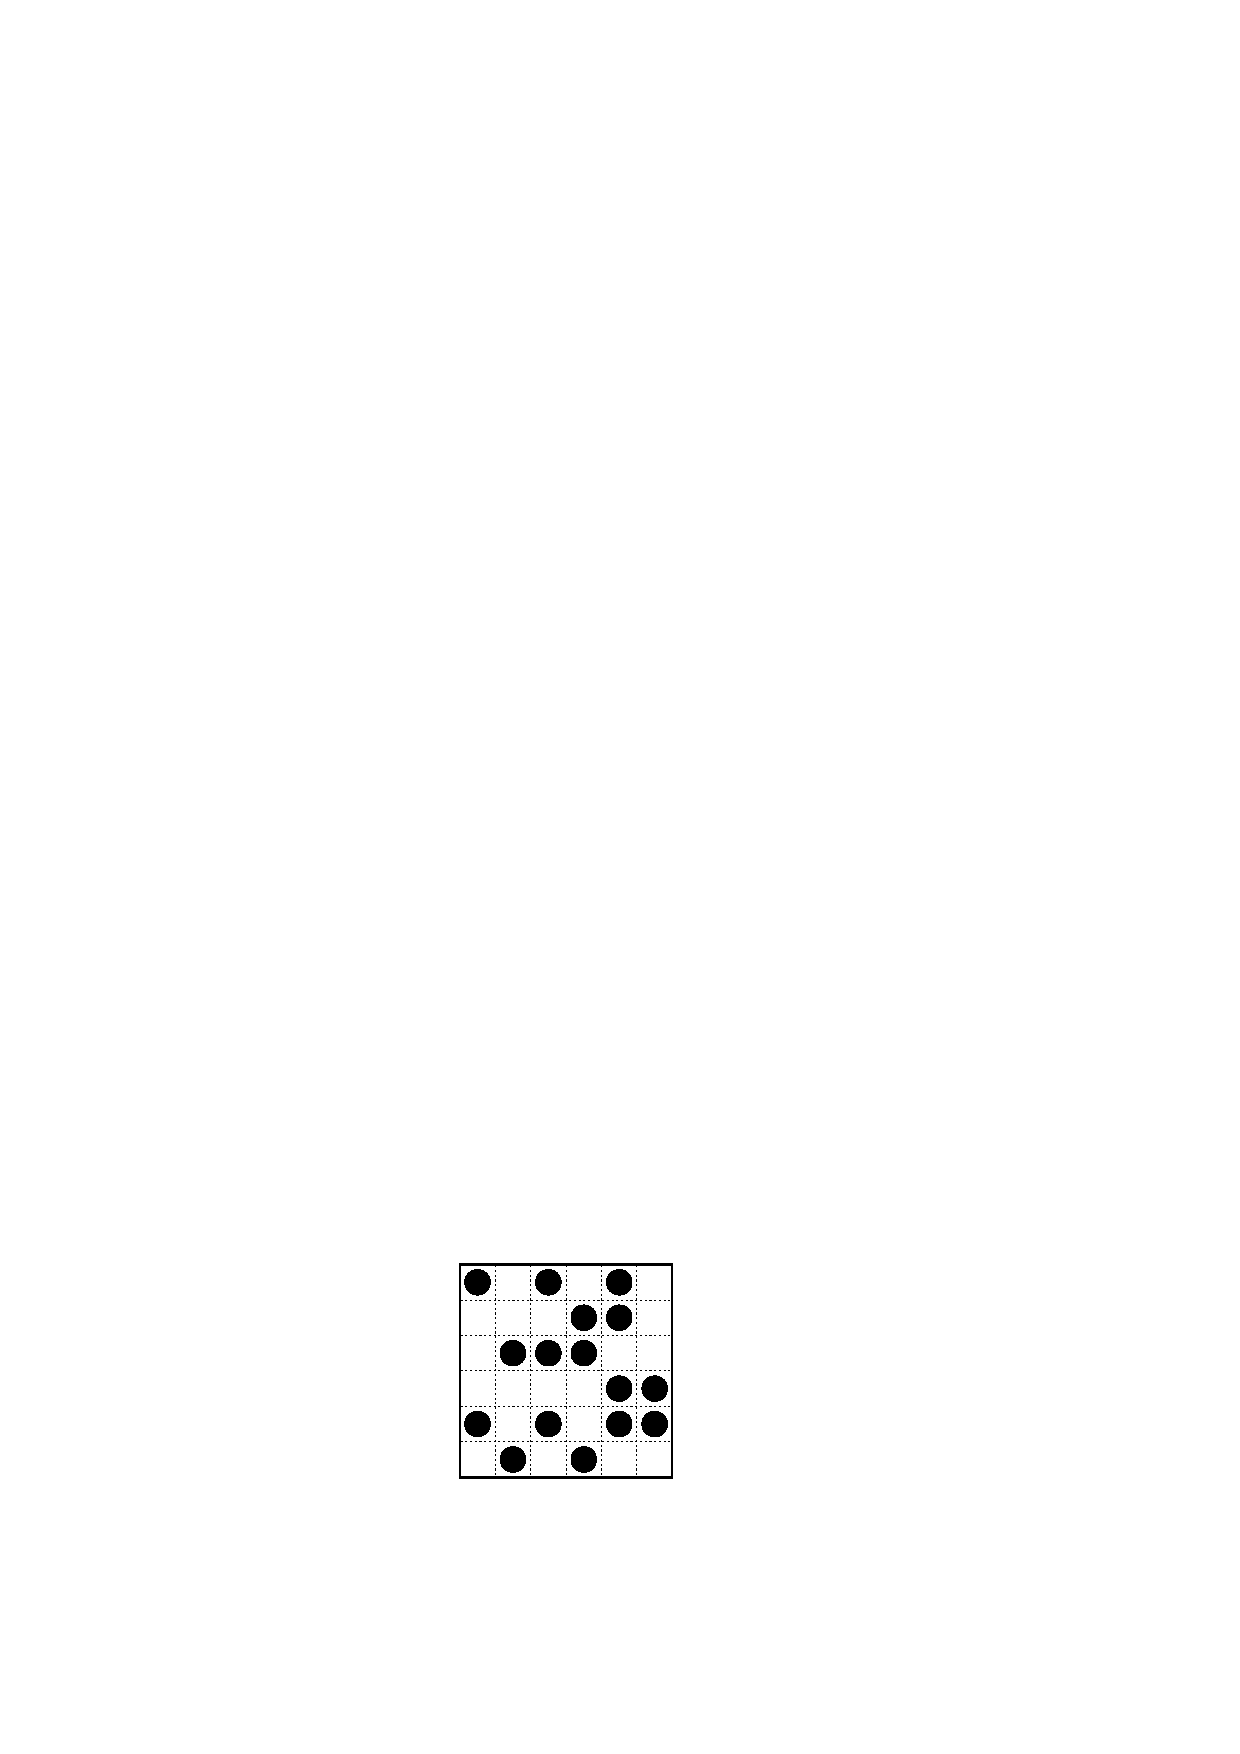
\includegraphics[width = .3\textwidth]{Fig1.pdf}
\caption{格点,黑色为占据}\label{Fig1}
\end{figure}



\section{Ising model}

在固体中,我们通常会遇到晶格结构,这些晶格结构很大程度上促使我们把系统想象为处于格点上。不需要严格的量子力学的情况下我们实际上就已经接触过这种描述了:Ising model。考虑一个晶格,上面格点标号$i$。每一个格点上面有一个变量$\sigma_i$,只有两个分立的取值$\sigma_i=\pm1$。Ising model认为,系统的Hamiltonian可以很好地描述为
\begin{align}
H=-J\sum_{\langle i,j\rangle}\sigma_i\sigma_j
\end{align}

\end{document}
